\documentclass[10pt,twocolumn,letterpaper]{article}

\usepackage{cvpr}
\usepackage{times}
\usepackage{epsfig}
\usepackage{graphicx}
\usepackage{amsmath}
\usepackage{amssymb}
\usepackage{mathrsfs}
\usepackage{multicol}
\usepackage{caption}

%%%%%%%%%%%%%%%%%%%%%%%% FEEDBACK %%%%%%%%%%%%%%%%%%%%%%%%
% This is the report, not the proposal. The report should emphasis different items, especially those
% listed in the grading criteria https://cseweb.ucsd.edu/classes/sp21/cse291-i/grading.html

% The first section of the paper should motivate the work. State the people problem (how working on
% this problem benefits people) and the technical problem. Then, state why previous solutions are
% inadequate, which you've done. Finally, state the research question that the paper your
% implemented answers and the proposed solution.

% Rather than cite/refer to the paper you're implementing, include enough details in your report
% that the reader understand what you've implemented and only has to look at the original paper if
% they want all the details.

% Provide a very brief description of SSIM and PSNR, since you're using these to evaluate your
% results and compare them to others.
%%%%%%%%%%%%%%%%%%%%%%%% FEEDBACK %%%%%%%%%%%%%%%%%%%%%%%%

%
% SECTIONS WE NEED
%

% Real world human problem (spatial resolution issue, why interpolating would help)

% Why interpolating is difficult 
% Why other approaches failed (we have this)

% More details on network and training process
% how this forces the network to estimate disparity

% Performance metrics
% Explain SSIM and PSNR (bigger is better)


% Include other packages here, before hyperref.

% If you comment hyperref and then uncomment it, you should delete
% egpaper.aux before re-running latex.  (Or just hit 'q' on the first latex
% run, let it finish, and you should be clear).
\usepackage[breaklinks=true,bookmarks=false]{hyperref}

\graphicspath{ {./images/} }

\cvprfinalcopy % *** Uncomment this line for the final submission

\def\cvprPaperID{6969} % *** Enter the CVPR Paper ID here
\def\httilde{\mbox{\tt\raisebox{-.5ex}{\symbol{126}}}}

% Pages are numbered in submission mode, and unnumbered in camera-ready
%\ifcvprfinal\pagestyle{empty}\fi
\setcounter{page}{1}
\begin{document}

%%%%%%%%% TITLE
% \title{Final Project Proposal - <Copy paste from Ravi>}
\title{Implementing Learning-Based Light Field View Synthesis}

\author{Thomas Lauer\\
UC San Diego\\
9500 Gilman Drive, San Diego CA\\
{\tt\small tlauer@ucsd.edu}
% For a paper whose authors are all at the same institution,
% omit the following lines up until the closing ``}''.
% Additional authors and addresses can be added with ``\and'',
% just like the second author.
% To save space, use either the email address or home page, not both
\and
Winston Durand\\
UC San Diego\\
9500 Gilman Drive, San Diego CA\\
{\tt\small wdurand@ucsd.edu}
}

\maketitle
%\thispagestyle{empty}

%%%%%%%%% ABSTRACT
\begin{abstract}
Light field photography allows for the capture of images from multiple
perspectives using a single camera array or array of microlenses. However
these come at a tradeoff between spatial resolution and angular resolution.
As the number of the microlens elements increases, the resulting lightfields
have higher angular resolution which is useful for depth estimation,
but will have lower spatial resolution for novel view synthesis.
We implement the a paper on learning based method to synthesize views from light
field camera data \cite{LearningViewSynthesis} in PyTorch.
\end{abstract}

% GUIDELINES for proposal:
% a list of four to six milestones, and deadlines to achieve the milestones
% a list of questions to be answered during the project and discussed in the report
% if the project is experimental, which existing software you will use directly or build upon
% if the project is experimental, precisely which datasets you will use and where you can obtain them quickly
% a few recent and very closely related papers that you will build on, with full bibliographic data.

%%%%%%%%% BODY TEXT
\section{Introduction}

Standard images are can be parameterized by an irradiance function $L(\theta, \phi)$, which
describes the light entering a camera from a certain angle $(\theta, \phi)$. Light fields
extend this to add a spatial component, $L(x, y, z, \theta, \phi)$ or $L(x, y, \theta, \phi)$. 
These two representations are equivalent if the radiance of a ray remains constant along its length,
which is a valid assumption for rays travelling through air.

Lytro is a commodity light field camera which uses microlenses to capture multiple
perspectives of a scene on one image sensor. The sensors of light field cameras have a 
limited resolution, and a tradeoff must be made between capturing more views of the scene 
(by densely sampling $x$, $y$, and $z$ in spatial resolution), or increasing the resolution of each view 
(by densely sampling $\theta$ and $\phi$). 
Lytro samples approximately $14 \times 14$ views of the scene, each with a resolution of 541 by 376 pixels.
However, many of the edge outer views contain invalid data, so we focus on the center $8 \times 8$ section.
The resolution of each view is much lower than consumer cameras, 
and contributed to the slow adoption of light field cameras in consumer products.

If the camera could sample only the corner 4 views and reliably interpolate the ones in between, each individual view
could be of a much higher resolution. This would also lower the cost of light field cameras by reducing the required
sensor resolution. Alternatively, phones with multiple cameras could use each camera as a 
view of the scene, and create light fields with no additional hardware. 

\section{Current Work}

% Insert summary of levoy 96 (this bit is related) (needs proper citation)
Kalantari summarizes several existing methods for interpolating lightfields and their drawbacks.
Many rely on high quality input images and well defined orientations between views,
which are difficult to achieve with consumer light field cameras, and impossible with light fields
captured by hand with cellphone cameras.

Many geometric methods novel view synthesis 
such as Levoy \etal~\cite{levoy1996light} require relatively high sample counts to ensure full
coverage of the 4D lightfield, as the simple linear interpolation used by Levoy
do not work well if there are heavily occluded regions or missing data.

Wanner \etal~\cite{Wanner} utilizes an optimization based approach, which calculates disparities
using traditional computer vision as a preprocessing step. However, because the disparity estimation
is independent from the loss function, it can not be optimized as part of the training process. 

Kalantari \etal~\cite{LearningViewSynthesis} propose a method to interpolate between 
sparsely sampled sub-apertures views. They use an $8 \times 8$ subset of the full $14 \times 14$ subaperture, since the
edge pixels are often black. The four corner sub-aperture views are fed into a series of two 
networks, the first is used to predict disparity which is then used to warp the sample images to the final perspective.
The second network then takes these warped images, along with some additional metadata, and blends them together
to produce the final RGB image of the novel view. Keeping this process differentiable allows both CNNs to 
be trained at the same time, which lets the disparity estimator become tuned to work with the final CNN.

\section{Technology}

We implemented this using PyTorch, because it has high performance,
automatically handles calculating derivatives, and we have previous experience with it.
In addition, we used NumPy to compute the preprocessing and feature extraction of the input lightfields,
and SciPy for the image quality metrics.

\section{Dataset}

We train our model using using Lytro captures since they represent a regularized input format with
online datasets easily available. In this paper, we make use of the Standford Lytro dataset by Raj \etal~\cite{StanfordLytro}
Further, Lytro captures are ideal for our purposes since it contains a large number of separate views between the
four corner images we use. Our dataset is comprised of 68 images primarily from their flowers and plants dataset with
other from occlusions and miscellaneous. Because Kalanatri \etal noted their implementation had issues with thin occlusions
we intentionally decided to do a large amount of our training on flowers and plants since those tended to have a large number
of thin, complex occlusions for the network to learn to interpret. A full list of the images used for training and
validation is included in our supplemental code.

\section{Implementation Details}

Our implementation closely follows that of Kalantari \etal~\cite{LearningViewSynthesis} with several modifications such
as being based on PyTorch \cite{PyTorch}.

\subsection{Preprocessing}

Each lightfield is cropped to only use the inner $8 \times 8$ grid of images out of the total $14 \times 14$ available
since the microlens actually captures a circle of data. For training, we additionally ignore the outer 60 pixels where
undesirable artifacts sometimes occur and train on $60\times60$ patches with a stride of 24 pixels to ensure overlap.
Each patch has its depth data estimated for all 64 ground truths and is saved to disk. Across the 68 images from the
Stanford Lytro dataset by Raj \etal~\cite{StanfordLytro}, we synthesize roughly 600,000 unique patch views total split
90/10 between training and validation passes.

For the disparity features, we estimate 100 disparity levels over a $[-21, 21]$ pixel window using the process from Tao \etal~\cite{tao2013depth}.
After backwarping each of the four corner images to the target location, we compute the mean and average at each pixel across the four warped images
for that disparity level. All of these features are then packaged into a $200 \times H \times W$ array to be fed into the disparity network.

\subsection{Network}

Our network was implemented using PyTorch, using two separate convolutional networks to perform the
disparity estimation and final color assembly. Our disparity estimation network takes a 
$200 \times H \times W$ tensor as input, which we calculate using the preprocessing step.

Here is the architecture of the disparity estimation network.

\begin{center}
\begin{tabular}{|c c c c|}
    \hline
    Input & Output & Kernel Size & Activation \\
    \hline
    200 & 100 & $7 \times 7$ & ReLU \\
    100 & 100 & $5 \times 5$ & ReLU \\
    100 & 50 & $3 \times 3$ & ReLU \\
    50 & 1 & $1 \times 1$ & None \\
    \hline
\end{tabular}
\end{center}


This disparity is then used to warp the 4 input views using the following equation:

$$
\overline{L}_{p_i} = L_{p_i} \left[ s + \left(p_i - q\right) D_q(s) \right]
$$

Where $s$ is the pixel location, $p_i$ is the location of the input view, and $q$ is the location of the
desired novel view. $D_q(s)$ is the estimated disparity at the pixel from the depth estimation network,
and $L_{p_i}(s)$ is the color of the novel view. We use the grid\_sample function from PyTorch, which integrates
with autograd to allow backpropagating the weights through $L_{p_i}(s)$. $s$, $p_i$, and $q$ are all 
constant precalculated inputs, and autograd is able to compute the derivative 
$\frac{\partial \overline{L}_{p_i}}{\partial D_q}$ automatically. 

These four RGB images, along with the $u$ and $v$ 
locations of the desired novel view and the disparity estimate from the first network are concatenated
together into a single 15 channel image. Kalantari \etal name this image $H$. This is used as the input to the color estimation network, which
has the following architecture:

\begin{center}
\begin{tabular}{|c c c c|}
    \hline
    Input & Output & Kernel Size & Activation \\
    \hline
    15 & 100 & $7 \times 7$ & ReLU \\
    100 & 100 & $5 \times 5$ & ReLU \\
    100 & 50 & $3 \times 3$ & ReLU \\
    50 & 3 & $1 \times 1$ & None \\
    \hline
\end{tabular}
\end{center}

Because none of the convolutions have padding, the network loses 12 pixels on each edge, reducing
the $60 \times 60$ patches during training to $36 \times 36$. Training without padding is ideal in this situation, 
because it would make the training patches less representative of the entire image.

\subsection{Training}

\begin{figure*}
\begin{center}
\begin{tabular}{|l | c c c c|}
    \hline
    Network & Feature Extraction & Disparity & Color Features (Warp) & Color Network \\ \hline
    Reference (4x CPU) & 3.19s & 4.52s & 0.13s & 1.52s \\
    Ours (1x CPU) & 1.3s & 6.62s & 0.09s & 1.85s \\
    Ours (GPU) & 1.3s (CPU) & 0.104s & 0.0044s & 0.024s \\ \hline
\end{tabular}
\caption{Execution time of their Matlab implementation and our PyTorch implementation.}
\end{center}
\end{figure*}

Our loss function is directly the $\mathcal{L}_2$ distance between the channel-wise RGB values of the novel image
and the ground truth image. While Kalantari \etal needed to numerically calculate the gradient of the interpolation
step which warps the ground truth images to the novel viewpoint, PyTorch's autograd is able to handle this automatically.
We needed to be careful to not destroy the gradient chain while calculating $s + \left(p_i - q\right) D_q(s)$, which had
to be done manually outside of a PyTorch function, because autograd builds the sequence of 
operations to backpropegate gradients on.

Additionally, we used the ADAM optimizer with a learning rate of $1e-4$, $\beta_1 = 0.9$, $\beta_2 = 0.999$, and $eps = 1e-8$.
We evaluate our training loop on batches of 64 $60 \times 60$ pixel patches. 
Our training loop runs on 8951 batches, which gives a total of 553,664 patches and over 700 million
individual pixels to train on. 
This is significantly more data than the roughly 100,000 patches Kalanatri \etal trained and their roughly 100 million samples.
Our implementation is also significantly faster than theirs, it took their network 12.3 seconds to generate a novel viewpoint
whereas ours takes 6.2 seconds. We believe this is mostly because of improvements in hardware from 2016, and has little to do with the
actual algorithms. We trained the final version of our network for 69 epochs over the course of approximately 24 hours cumulatively.

\section{Results}

\begin{center}
Flowers and Plants 25

\begin{tabular}{|c c c|}
    \hline
    Network & SSIM & PSNR \\ \hline
    Ours & 0.935 & 33.615 \\
    Reference & 0.931 & 33.19 \\ 
    \hline
\end{tabular}
\end{center}
            
\begin{center}
Rocks

\begin{tabular}{|c c c|}
    \hline
    Network & SSIM & PSNR \\ \hline
    Ours & 0.932 & 31.46 \\
    Reference & 0.969 & 34.66 \\ 
    Wanner and Goldluecke & 0.488 & 16.57 \\
    \hline
\end{tabular}
\end{center}

\begin{center}
Average

\begin{tabular}{|c c c|}
    \hline
    Network & SSIM & PSNR \\ \hline
    Ours & 0.953 & 35.67 \\
    Reference & 0.957 & 35.99 \\ 
    \hline
\end{tabular}
\end{center}

\begin{figure*}[p]
    \begin{multicols}{3}
        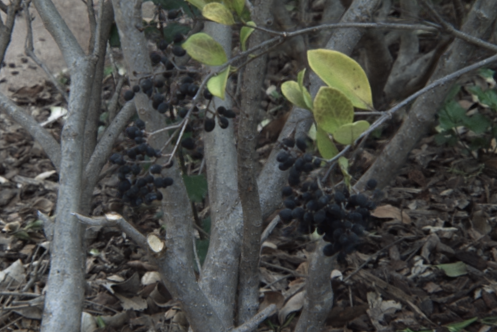
\includegraphics[width=\linewidth]{flowers_25/kalantari_05_05.png}
        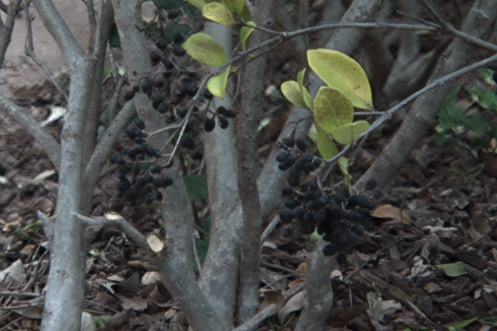
\includegraphics[width=\linewidth]{flowers_25/ours_05_05.png}
        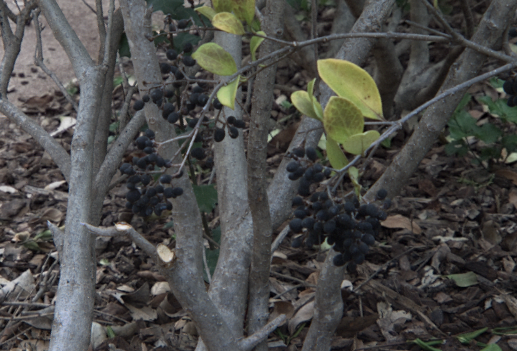
\includegraphics[width=\linewidth]{flowers_25/truth_05_05.png}
    \end{multicols}
    \begin{multicols}{3}
        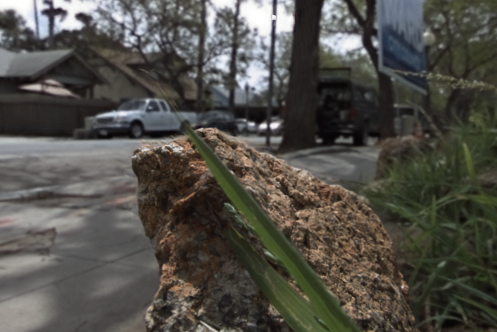
\includegraphics[width=\linewidth]{rock/kalantari_05_05.png}\par\caption*{Kalanatri \etal}
        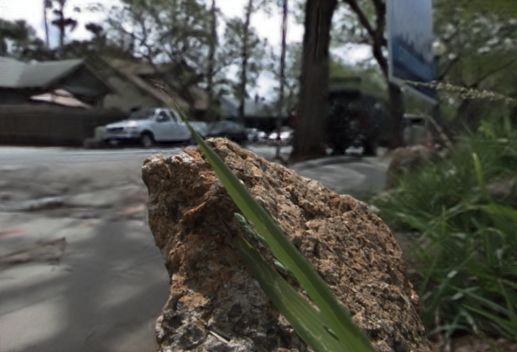
\includegraphics[width=\linewidth]{rock/ours_05_05.png}\par\caption*{Our Results}
        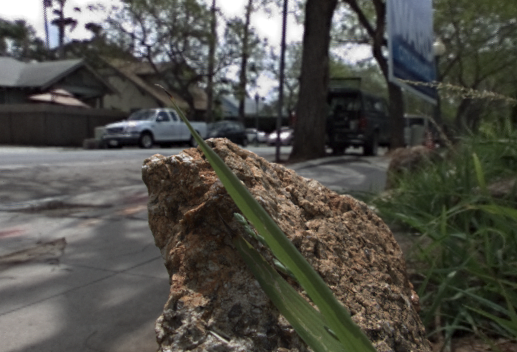
\includegraphics[width=\linewidth]{rock/truth_05_05.png}\par\caption*{Ground Truth}
    \end{multicols}
    \begin{multicols}{2}
        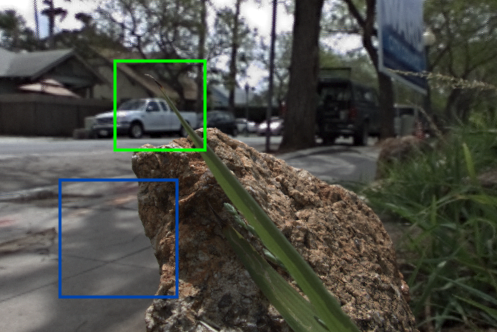
\includegraphics[width=\linewidth]{truth_05_05_map.png}
        \begin{multicols}{3}
            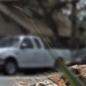
\includegraphics[width=\linewidth]{rock_crop_leaf/kalantari_05_05.png}\par\vspace{0.1in}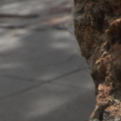
\includegraphics[width=\linewidth]{rock_crop_walk/kalantari_05_05.png}\par\caption*{Kalantari \etal}
            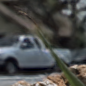
\includegraphics[width=\linewidth]{rock_crop_leaf/ours_05_05.png}\par\vspace{0.1in}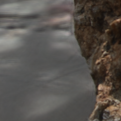
\includegraphics[width=\linewidth]{rock_crop_walk/ours_05_05.png}\par\caption*{Ours}
            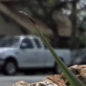
\includegraphics[width=\linewidth]{rock_crop_leaf/truth_05_05.png}\par\vspace{0.1in}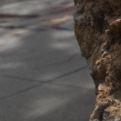
\includegraphics[width=\linewidth]{rock_crop_walk/truth_05_05.png}\par\caption*{Ground Truth}
        \end{multicols}    
    \end{multicols}
    \caption{
        Here we compare the results from Kalantari \etal's implementation, our implementation, and the ground
        truth image at view (5, 5). We chose to compare this view since it is one of the farthest from the
        corner views. The two network's performance is very comperable, and both were able to recover some
        features the other was not. Our network was able to reconstruct the thin leaf, while we struggled with
        the large patches of relatively low detail, such as the the sidewalk in the lower left corner. This was
        a pattern which was prevalent the images we tested reconstruction on.
    }
\end{figure*}

\begin{figure*}[p]
    \begin{multicols}{2}
        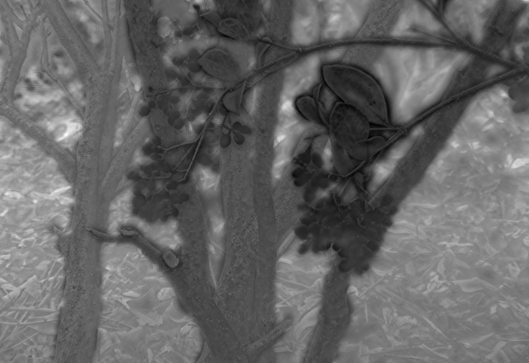
\includegraphics[width=\linewidth]{flowers_25/ours_05_05_disp.png}\par\caption*{Our Generated Disparity}
        
\includegraphics[width=\linewidth]{flowers_25/stanford_depth.png}\par\caption*{Stanford Lytro Archive Depth}
    \end{multicols}
    \caption{
        This is a comparison between our generated disparity map and the depth map from the Stanford Lytro Archive.
        The disparity map from the network has a halo effect around the edges of objects, we believe these are areas where changes
        in the image warping can have a heavy effect on our $\mathcal{L}_2$ loss function. Regions of contiguous color
        would be less sensitive to changes in warping, and therefore we expect they would be penalized less heavily.
        However, this does not need to be true disparity, just what the color estimation network needs to reconstruct the final image.
    }
\end{figure*}

When evaluating the effectiveness of our network, we elected to use both the structural similarity index measure (SSIM)
and Peak signal-to-noise ratio (PSNR) to compare results to the ground truth capture. SSIM represents the similarity
between a distorted and distortion free image, and is a value in the range 0 to 1, where 1 indicates perfect retention
of perceptual quality compared to the ground truth data. PSNR is the ratio between the maximum intensity of the image
and the noise introduced by reconstruction. Each result and ground truth image was additionally cropped so any
non-captured pixels around the edges would not be included in our metrics.

We computed the PSNR and SSIM scores for all views of 4 different light fields, giving us 256 views to compare.
These scores were averaged to compute the average PSNR and SSIM of the two networks. 


We created a series of animations to compare our results to Kalantari \etal's. These can be viewed 
\href{https://drive.google.com/drive/folders/1DDbB1v1vbq7zsg3srJPDKFlI9H7mGEmC?usp=sharing}{here}.

\section{Conclusions and Future Work}

In the future, there is potential to further improve this system with varied input views and synthesized
view depth. Additionally, the depth estimation used at present is not entirely scale agnostic as it
uses a pixel based window for disparity estimation. This can definitely be adjusted to be more resolution
independent as is on of the reasons we were unable to test it on data from the Stanford lightfield array.

While we initially wanted to generate out of plane images with this technique, we realized that our training dataset
of Lytro light fields has no ground truth information for out of plane images. This means that we can not directly
train our network to produce out of plane images. However, this network could be used to densely sample a sparse light field,
and a more traditional approach could be used to generate the out of plane images.


{\small
\bibliographystyle{ieee_fullname}
\bibliography{egbib}
}



\end{document}
